%!TeX spellcheck = es_ES

Este apartado se estructurara de la siguiente forma: Primero en la motivación, se explican los motivos por los cuales se ha decidido dedicar el proyecto de final de grado a construir una aplicación \textit{backend} para la gestión de árboles genealógicos usando bases de datos NoSQL, más concretamente basadas en grafos, también como se ha decidido ofrecer el servicio a la aplicación para gestionar estos árboles. Después se expondrá el estado del arte donde se contextualizara el proyecto. A continuación, se analizará el estado en el que se encuentra la tecnología con la cual realizaremos el desarrollo de este proyecto. Y por último, se definirán los objetivos que se han perseguido alcanzar con la consecución de este proyecto.

\subsection{Motivación}
La rápida evolución de las tecnologías constantemente nos acerca nuevas formas de aproximarnos a problemas que ya estaban resueltos, ya sea para resolver el problema de una forma más eficiente, elegante y/o versátil, entendamos por elegante que conceputalmente la solución propuesta nos resulta sencilla de comprender en contraposición a otra más compleja y por versátil que la solución parte de una abstracción que puede ser aplicada para solucionar diferentes problemas. Bajo esta perspectiva se ha buscado desarrollar una plataforma \textit{backend} que nos permita gestionar un repositorio de árboles genealógicos almacenado en una base de datos orientada a grafos, mediante una API rest-ful. Durante el desarrollo de la introducción veremos como la decisión de resolver el problema de ''realizar un repositorio de árboles genealógicos en bases de datos orientadas a grafos`` y su gestión  mediante una API rest-ful nos ayuda a dar una solución eficiente, elegante y versátil.
\newpage
\subsection{Contextualización del proyecto}
Se empezara introduciendo los diferentes conceptos sobre los que se sustenta el proyecto y explicando su relación con el proyecto:

\subsubsection{Los árboles genealógicos}
Un arbole genealógico, también llamado genorama, es la representación gráfica de los antepasados  y descendientes de un individuo.Para su representación  se suelen usar tablas o árboles, siendo esta última la forma más común.

\textbf{Uso y aplicación de los árboles genealógicos}\newline
Los árboles genealógicos se usan como herramienta en la genealogía, que se encarga de estudiar y seguir la ascendencia y descendencia de una persona o familia. La genealogía es una ciencia auxiliar de la Historia y es trabajada por un genealogista. Uno de los objetivos del software a desarrollar es dar soporte a los genealogistas.\\ Por otro lado hay varias comunidades de aficionados que llevan sus propios árboles genealógicos, el software creado también les podrá dar servicio a esta tipología de usuarios.

\paragraph{GEDCOM \cite{aboutGEDCOM} (\textbf{GE}nealogical \textbf{D}ata \textbf{COM}munication)}.\newline
Es un formato de archivo de datos, proporciona un formato flexible y uniforme para el intercambio de datos genealógicos computarizados. El modelo de datos que usa GEDCOM esta basado en los núcleos familiares y individuos. En el siguiente apartado donde abalaremos de las tecnologías usadas para desarrollar el proyecto entramos en detalle de las cuestiones técnicas del formato, profundizando en su modelo de datos y su estructura.

\subsubsection{Bases de datos orientadas a grafos (BDOG)}
\label{sec:bdog}
Las bases de datos orientadas a grafos se investigan desde hacer mucho, su poca popularidad es debido a la imposición generalizada del modelo relacional, este fenómeno pudo ser producido por la simplicidad y fácil manejo del modelo relacional.

Con la aparición de las nuevas metodologías ágiles y el requerimiento de modelos que permitan mayor flexibilidad en el desarrollo (e.g. SCURM) y las exigencias de velocidad de nuevas plataformas con modelos donde los datos están altamente asociativos y las consultas requieren usar gran cantidad de estas asociaciones o relaciones (e.g. redes sociales) las BDOG han ganado popularidad. Los motivos por los que estas bases de datos satisfacen los requerimientos mencionados se explican en los siguientes apartados. A continuación se explica las entidades que conforman una BDOG.

\paragraph{Estructura}.\newline
Una DBOG representa la información como nodos de un grafo y sus relaciones mediante sus aristas. Lo que resulta realmente diferencial del modelo relacional es que en este modelo las relaciones son ciudadanos de primer orden de la estructura del grafo (i.e. A diferencia de una base de datos relacional, donde las claves foráneas que relacionan los objetos del modelo son atributos de estos.)\cite{graphdbbook}, lo que repercute en que las consultas con un alto nivel de acoplamiento sean más rápidas, los motivos de este fenómeno se explicaran más adelante. 
\paragraph{Propiedades}.\newline
Hay dos propiedades principales de las BDOG que tenemos que considerar a la hora de entender sus capacidades:
\begin{description}
\item[Forma de almacenado subyacente].\newline
Solo algunas BDOG almacenan la información de forma nativa en una estructura de grafo, otras por lo contrario serializan los datos a un modelo relacional o algún otro modelo de almacenamiento de datos de propósito general.
\item[Motor de procesamiento].\newline
Una propiedad de las BDOG es la adyacencia libre de indices, esto quiere decir que los nodos están conectados físicamente entre ellos en la base de datos. Esto mejora la eficiencia en las consultas que han de recorrer nuestro modelo, lo que provocaría que en una base de datos relacional tuviésemos que hacer una gran cantidad de \textit{joins}. La contrapartida de la adyacencia libre de indice es que aumenta el coste de las consultas que no requieran recorrer nuestro modelo. Existen técnicas en el diseño de nuestros  modelos que nos permiten esquivar esta contra-prestación convirtiendo atributos de los nodos en nuevos nodos y simulando indices sobre estos atributos \cite{rodriguez2010graph}.
\end{description}

\paragraph{Expresividad y simplicidad}.\newline
La propiedad de las BDOG donde las relaciones son ciudadanos de primer orden, a diferencia de otras bases de datos como las SQL que usan el modelo relacional donde las relaciones se definen mediante claves foráneas entre los datos o otras aproximaciones como las bases de datos basadas en clave-valor donde las relaciones tampoco son ciudadanos de primear orden, nos permite definir modelos simples y expresivos sobre nuestro domino.\newline

La figura \ref{fig:grdb} nos da una visión de algunas de las tecnologías de BDOG más importantes que podemos encontrar hoy en día, el valor de \textit{Graph Processing} se mide según si la tecnología hace uso de la adyacencia libre de indices en su motor de procesamiento y el \textit{Graph Storage} se evalúa como nativo o no nativo si la base de datos usa seralizadores para acabar almacenando los dato en una estructura no grafoide (i.e SQL o clave-valor).

\begin{figure}[ht!]
\center
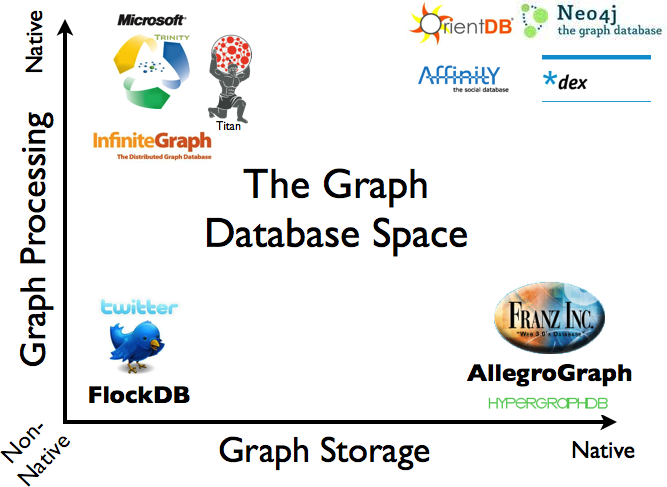
\includegraphics{grdb.png}
\caption{Visión del conjunto de tecnologías}
\label{fig:grdb}
\end{figure}
\newpage

\subsubsection{REST-ful (REpresentational State Transfer)}
REST nace como un estilo de arquitectura del software que consiste en coordinar un conjunto de restricciones arquitectónicas  a los componentes, conectores y recursos, en un sistema distribuido de \textit{hypermedia}(e.g. imágenes, audio, vídeo, texto plano y hiperenlaces). Estas restricciones se efectúan con el objetivo de mejorar la escalabilidad, simplicidad, modificabilidad, visibilidad, portabilidad, rendimiento y confiabilidad.\\
Los sistemas que se adecuan a una arquitectura rest son llamados rest-ful. Estos sistemas se comunican a través de HTTP con el uso de los verbos que esté implementa, normalmente los verbos GET, POST, PUT, DELETE suelen estar asimilados a las operaciones CRUD de una base de datos.
Las interfaces que usan estos sistemas son llamados \textit{endpoints}(i.e URIS).
En la actualidad existen varios \textit{frameworks} orientados al desarrollo de APIs REST, más adelante haremos un estudio de algunas de las diferentes tecnologías que podemos encontrar.

\subsection{Perspectiva general del software genealógico actual.}

Todo software genealógico, como mínimo permite almacenar la siguiente información de un individuo: datos personales (nombre, apellidos, etc), información de los eventos vitales de la misma (fechas y lugares de estos eventos) y las relaciones (familiares) entre personas.  Contra más flexible es el programa más información te permite introducir acerca de un individuo. También proporcionan diferentes maneras de representar la información y permiten exportar a GEDCOM la información representada y importar archivos GEDCOM.

La mayor parte del software genealógico actual esta basado en soluciones de escritorio, pero en los últimos años han proliferado diferentes soluciones web como myheritage o familysearch, que no solo sirven como plataforma de edición sino que también son grandes plataformas \textit{cloud} en las que se almacenan los árboles genealógicos.

Las soluciones más avanzadas, aparte de la gestión de árboles también ofrecen herramientas más orientadas a la investigación, como podrían ser sistemas de búsqueda de individuos basados en sus relaciones o herramientas estadísticas.

\subsection{Análisis previo de tecnologías}

\subsubsection{Base de datos}
Para la selección de las bases de datos han valorado las siguientes bases de datos orientadas a grafos, estas bases de datos han estado seleccionadas bajo criterios subjetivos buscando que aportasen rasgos diferenciales entre ellas, pero a la vez se pueda acceder a documentación o soporte para problemas específicos un una cierta facilidad:

\begin{description}
\item[HyperGraphDB (\url{http://hypergraphdb.org/})]:
\\Es un base de datos orientada a grafos de propósito general, extensible, potable, distribuida y integrable. Diseñada especialmente para proyectos sobre inteligencia artificial y web semántica. También se pude usar como base de datos orientada a objetos.
\item[InfoGrid (\url{http://infogrid.org})]:
\\Es una base de datos orientada a grafos especialmente enfocada al desarrollo de aplicaciones \textit{backend} REST-ful. Hace especial énfasis en la orientación a objetos. De este proyecto destaca su modularidad. 
\item[Neo4j (\url{http://neo4j.com/})]:
\\Esta base de datos basada en grafos esta diseñada como una base de datos de propósito general, cumple los requisitos de las dos anteriores a pesar que no se pueden crear hyperedges como tal a diferencia de HyperGraphDB, por otro lado se pueden usar técnicas en la representación de los grafos que los simulan. También aporta mejoras en el almacenamiento de los datos respecto a InfoGrid, ya que el almacenamiento esta implementado en grafos de forma nativa.
\end{description}

\textbf{Decisón}:\\
Finalmente se ha escogido Neo4j las principales razones son:
\begin{itemize}
\item Neo4j almacena los datos en un grafo de forma nativa.
\item El motor de procesamiento es orientado a grafos.
\item Es una de las bases de datos orientadas a grafos más usadas por ello con más comunidad. (fuente \href{http://db-engines.com/en/ranking}{DB Engines Ranking})
\item A pesar de usar un lenguaje especifico, Cypher es muy intuitivo ya que usa una representación grafoide para realizar las consultas.
\end{itemize}.


\subsubsection{Lenguaje de programación}
Los lenguajes escogidos para el análisis han estado seleccionados con criterios subjetivos, seleccionándolos de tal forma que aporten alternativas a la hora tanto de dar agilidad a la implementación como a ser eficientes en el rendimiento. También se ha tendió en cuenta los \textit{frameworks} que se pueden usar en estos lenguajes para la consecución de una API rest.\\Para desarrollar este proyecto se ha optado entre los siguientes lenguajes de programación.

\begin{description}
\item[Scala (\url{www.scala-lang.org/})]:
\\Scala es un lenguaje de propósito general multi-paradigma, da soporte completo para programación funcional y orientada a objetos, también dispone de un sistema de inferencia de tipo estático muy potente. Se compila a Java byte code y se ejecuta sobre la maquina virtual de Java. Es totalmente interoperable con Java por lo que se pueden usar librerías Java y viceversa.

Frameworks:

\begin{description}
\item[Scarlata(\url{www.scalatra.org/})]:
\\Es un \textit{Micro-framework} para scala, consta de librerías para la creación de una API rest completa, como \textit{micro-framework} no fuerza ningún tipo de arquitectura. Se usa para desarrollar bajo la siguiente filosofa:

\begin{description}
\item[Empezar desde lo pequeño, desarrolla hacia arriba]: \\Empieza construyendo un pequeño núcleo y integra módulos simples para solucionar las tareas.
\item[Libertad]: \\Permite al programador usar la estructura y las librerías que crea convenientes para su aplicación.
\item[Solido pero no terco]: \\Usa componentes sólidos para la creación de la API, por ejemplo, los serverlets no son una solución muy moderna a la gestión de la comunicación cliente servidor, pero tienen una gran comunidad detrás y son extremadamente estables. Por otro lado se anima a usar la flexibilidad del framework para usar nuevas técnicas y aproximaciones en diferentes ámbitos del servicio. 
\item[Ama HTTP]: \\HTTP es un protocolo de naturaleza carente de estado, no se ha de pretender usar mecanismos complejos que den la apariencia de estado.
\end{description}

\item[Lift(\url{liftweb.net/})]:
\\Es un \textit{framework} para scala, esta diseñado para seguir la arquitectura 'View First". Clama ser uno de los \textit{frameworks} más seguros y destaca por los siguientes puntos:

\begin{description}
\item[Seguridad]: \\Lift es resistente a casi todas las vulnerabilidades comunes incluyendo la mayoría de la lista ``OWASP \textit{top 10} de".
\item[Amigable para el desarrollador]: \\Lisft esta diseñado para facilitar la creación de aplicaciones de forma rápida y sencilla.
\item[Escalable]: \\Esta diseñado para dar soporte a grandes cantidades de trafico.
\item[Modular]: \\El programa se compone de módulos, esto da mucha agilidad a la hora ampliar las funcionalidades de los proyectos y da una arquitectura muy limpia y fácil de mantener.
\end{description}
\end{description}


\item[Python(\url{python.org/})]:
\\Python es un lenguaje de propósito general, interpretad, y de tipado dinámico. Es un lenguaje multi-paradigma, combina la orientación a objetos con la programación funcional. A diferencia de escala la parte funcional no esta totalmente desarrollada ya que no permite valores inmutables o técnicas como curring. Python esta diseñado para agilizar el proceso de desarrollo y facilitar la legibilidad y comprensión del código.

Frameworks:
\begin{description}
\item[Falsk(\url{flask.pocoo.org/})]:
\\Es un \textit{micro-framework}, esta diseñado permitir el desarrollo de aplicaciones web de forma flexible. Consta de los siguientes herramientas:
\begin{description}
\item[-]Incorpora servidor y debugger
\item[-]Integra soporte para unit test
\item[-]Gestor de peticiones RESTful
\item[-]Usa Jinja2 templating
\item[-]Soporte para ``Cookies'' con seguridad
\item[-]Cumple al 100\% el WSGI 1.0 (Estándar para la comunicación de las aplicaciones con el servidor) 
\item[-]Basado en unicode
\item[-]Extensamente documentado
\end{description}

\item[Django(\url{www.djangoproject.com/})]:
\\Es un \textit{framework}, esta diseñado permitir el desarrollo de aplicaciones rápidamente y con una estructura limpia. Consta de diferentes capas que aportan seguridad la aplicación. Esta basado en la arquitectura modelo vista controlador. Entre sus virtudes destacan la gran facilidad para modular las aplicaciones y facilitar su integración y una comunidad muy extensa, también dispone de una documentación clara, bien estructurada y muy completa. Django destaca en su web estos tres puntos:
\begin{description}
\item[-]Ridicualemtne rapido de desarrollar
\item[-]Altamente seguro
\item[-]Escalabilidad asombrosa
\end{description}
\end{description}

\textbf{Decisión}:
Finalmente se ha escojido Django. Los motivos han sido:
\begin{description}
\item[Velocidad de desarrollo a coste de velocidad de ejecución]: Python es conocido por la rapidez que aporta al desarrollar, dado que es une lenguaje de muy alto nivel con multitud de librerías, por otro lado el usar Djando nos aporta gran parte de las librerías necesarias para desarrollar una aplicación de servidor que de servició REST. Por contra esta decisión repercute en que la velocidad de ejecución de escala en comparación con python es mucho mayor, se asumirá esta desventaja ya que la finalidad del proyecto no es llevar el producto a un entorno de producción real donde la velocidad de ejecución sea capital. 
\end{description}
A destacar:
\begin{description}
\item[Django Rest Framework]:\\Framework que se integra con Django y proporciona herramientas para facilitar la seralización, enrutamientó teniendo en cuenta el protocolo REST-ful, autorización y autenticación, creación de vistas para las operaciones CRUD, etc.
\item[Django OAuth Toolkit]:\\Conjunto de herramientas para crear autenticación y autorización con permisos, basado en el protocolo oAuth2.
\item[Celerys]:\\Librería de python que permite combinado con una tecnología \textit{``message broker''} permite crear tareas que realicen funcionalidades de la aplicación o crear tareas asíncronas.
\item[neomodel OGM(Object graph maper)]:\\Permite crear modelos en la base de datos neo4j basándose en los modelos de la aplicación.
\end{description}
\end{description}


\subsection{Integración de leyes y regulaciones}
Al desarrollar una aplicación \textit{backend} donde se almacenaran datos de usuarios y personas se tendrá que respetar la \textbf{Ley Orgánica 15/1999 de Protección de Datos de Carácter Personal (Lopd)}. Por ello se tendrá que tener en cuenta:

\subsubsection{Derecho de información}
El derecho de información esta regulado en la \textbf{Ley Org
ánica 15/1999 de Protección de Datos de Carácter Personal (Lopd)}. Regula las condiciones en que se ha  de recoger, tratar y ceder los datos personales, su fin es proteger la intimidad y demás derechos ciudadanos. Para adecuarse a esta ley, si un usuario introduce datos personales de otra persona se tendrá que se notificar de la posesión de estos datos al afectado y pedir su aprobación para su almacenamiento.

\subsubsection{Consentimiento del afectado}
EL articulo 6 de la Lopd, regula que para tratar datos personales se ha de tener el consentimiento expreso del damnificado, por ello al registrarse los usuarios tendrán que aceptar una licencia de acuerdo con el usuario final (EULA). Por el momento al ser una plataforma en fase beta donde no se registraran los usuarios no se redactara dicho acuerdo ni se realizara ninguna confirmación a la hora del registro.